\section{Konvergenz von Taylorreihen}
\subsection{Einführung}

In diesem Kapitel werden wir eine Formel für die Abweichung der Taylorentwicklung von der tatsächlichen Funktion angeben. Ausserdem werden wir untersuchen, unter welchen Bedingungen die Taylorentwicklung konvergiert.

\begin{LA}
	{}{}
	Verwenden Sie für diese Aufgabe \href{https://www.geogebra.org}{geogebra}.
	\begin{enumerate}
		\item Zeichnen Sie den Graphen der Funktion $f(x)=\ln(x+1)$. (Eingabe f(x)=ln(x+1))
		\item Erzeugen Sie in Geogebra das Taylorpolynom $n$-ten Grades an der Entwicklungsstelle $x_0  =0$ (Eingabe TaylorReihe(f,0,n))\\
		      Hinweis: Durch den Befehl wird ein Schieberegler für $n$ erstellt, mit dem Sie den Grad des Taylorpolynoms verändern können.
		\item Untersuchen Sie das Verhalten der Taylorapproximation für verschiedene Werte von $n$ im Intervall $n=1$ bis $n=15$. Was stellen Sie fest?\\
		      Hinweis: In den Einstellungen des Schiebereglers können Sie den Minimal- und Maximalwert sowie die Schrittweite anpassen.
		      % \item 	Berechnen Sie die Differenz zwischen der Funktion $f$ und der Taylorentwicklung an den Stellen
		      %       \begin{enumerate}
		      % 	      \item $x=0.5$
		      % 	      \item $x=1$
		      % 	      \item $x=2$
		      %       \end{enumerate}
		\item 	Untersuchen Sie die Gleichung der unendlichen Taylorentwicklung von $f$ und argumentieren Sie, wieso die Reihe $T(2)$ divergiert.


	\end{enumerate}

\end{LA}
\clearpage
Die Taylorentwicklung einer Funktion $f$ ist in der Regel eine unendliche Summe, auch Reihe genannt. Solche Reihen können konvergieren oder auch nicht. Betrachten Sie dazu die folgenden Beispiele.
\begin{bsp}
	{Drei Beispiele für Taylorentwicklungen}{}
	\begin{enumerate}
		\item Die Taylorentwicklung von \(f(x) = \sin(x)\) lautet
		      \[T(x) = x - \frac{1}{3!}x^3 + \frac{1}{5!}x^5 - \frac{1}{7!}x^7 + \frac{1}{9!}x^9 \pm \ldots = \sum_{k=0}^{\infty} \frac{(-1)^k}{(2k+1)!} x^{2k+1}\]

		      Diese Reihe konvergiert für jedes \(x \in \mathbb{R}\) gegen \(\sin(x)\).
		\item Die Taylorentwicklung der Funktion \( f(x) = \begin{cases} e^{-\frac{1}{x^2}}, & \text{falls } x > 0 \\ 0, & \text{falls } x \leq 0 \end{cases} \) lautet
		      \[ T(x) = 0. \]

		      Offensichtlich konvergiert \( T(x) \) für jedes \( x \in \mathbb{R} \). Der Grenzwert 0 stimmt aber für alle \( x > 0 \) nicht mit dem Funktionswert überein.
		\item Die Taylorentwicklung von \( f(x) = \ln(1+x) \) ist
		      \[ T(x) = x - \frac{x^2}{2} + \frac{x^3}{3} - \frac{x^4}{4} \pm \ldots = \sum_{k=1}^{\infty} \frac{(-1)^{k+1}}{k} x^k \]

		      Wenn \( |x| > 1 \) ist, erhält man eine divergente Reihe. Für \( |x| < 1 \) hingegen konvergiert die Reihe gegen \( \ln(1+x) \).

	\end{enumerate}
\end{bsp}
Zusammengefasst erhalten wir folgenden Satz:
\begin{satz}
	{Konvergenz von Taylorreihen}{}
	Sei $T(x)$ die Taylorentwicklung einer Funktion $f$. Dann gibt es für jedes Argument $x$ drei Möglichkeiten:
	\begin{enumerate}
		\item Die Reihe $T(x)$ konvergiert und der Grenzwert ist $f(x)$
		\item         Die Reihe $T(x)$ konvergiert und der Grenzwert ist nicht $f(x)$
		\item
		      Die Reihe $T(x)$ divergiert
	\end{enumerate}

\end{satz}
\emph{Bemerkung}: Für die meisten Funktionen, die Sie kennen, gilt der erste Fall.

Will man eine Funktion durch ihre Taylorreihe darstellen, muss man also im Grunde zuerst beweisen, dass letztere wirklich konvergiert und dass der Grenzwert mit dem Funktionswert übereinstimmt.
Die Idee beim Beweis der Konvergenz einer Taylorreihe ist die, dass man die Abweichung der Taylorentwicklung $n$-ten Grades von dem tatsächlichen Funktionswert angibt, und anschliessend zeigt, dass diese Abweichung für wachsende $n$ gegen Null strebt.

\begin{definition}
	{Das $n$-te Restglied}{}
	Sei $T_n$ das Taylorpolynom $n$-ten Grades der Funktion $f$. Dann nennt man die Funktion
	$$R_n (x)=f(x)-T_n (x)$$
	das $n$-te Restglied der Taylorentwicklung.

\end{definition}
In anderen Worten: Das Restglied ist der Fehler, den man macht, wenn man die Funktion durch das Taylorpolynom $n$-ten Grades approximiert. Die folgenden vier Bilder zeigen die Sinusfunktion (blau), deren Taylorpolynom vom Grad $n=1, 3, 5, 7$ (orange), den Fehler $R_n(4)$ an der Stelle $x=4$ (rote Strecke) und der Verlauf der Funktion $y=R_n(x)$ (grün).

\begin{figure}[h!]
	\centering
	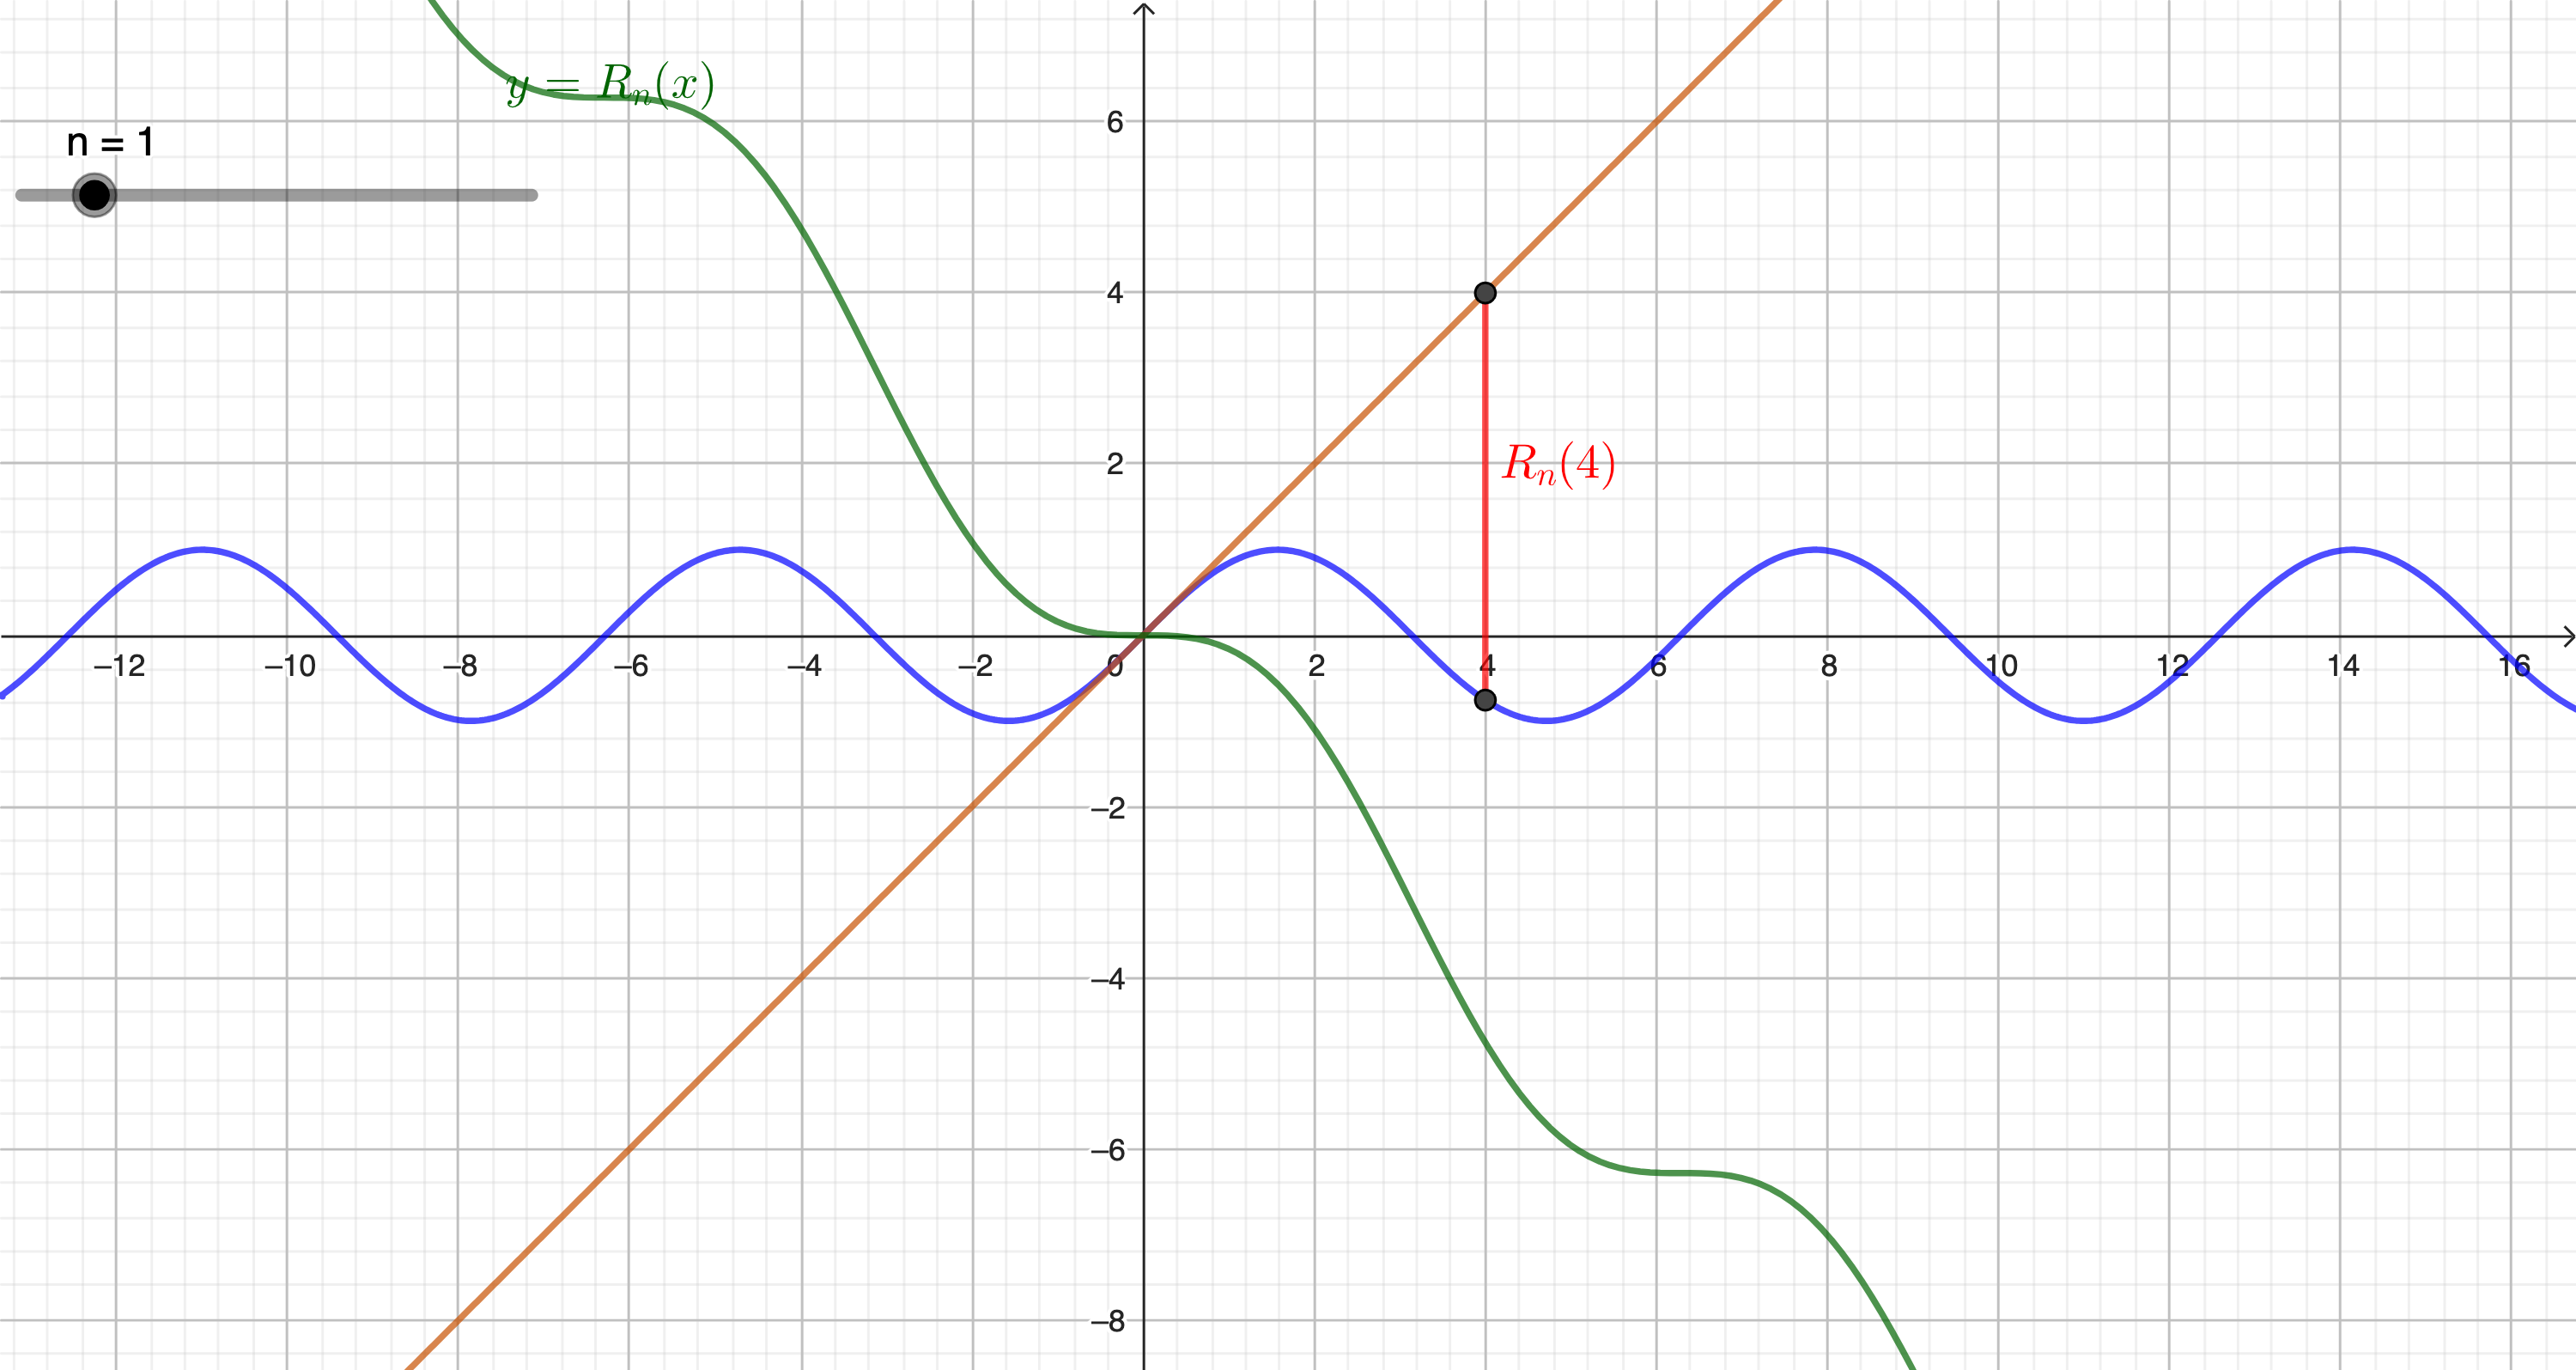
\includegraphics[width=0.45\textwidth]{media/restglied1.png}
	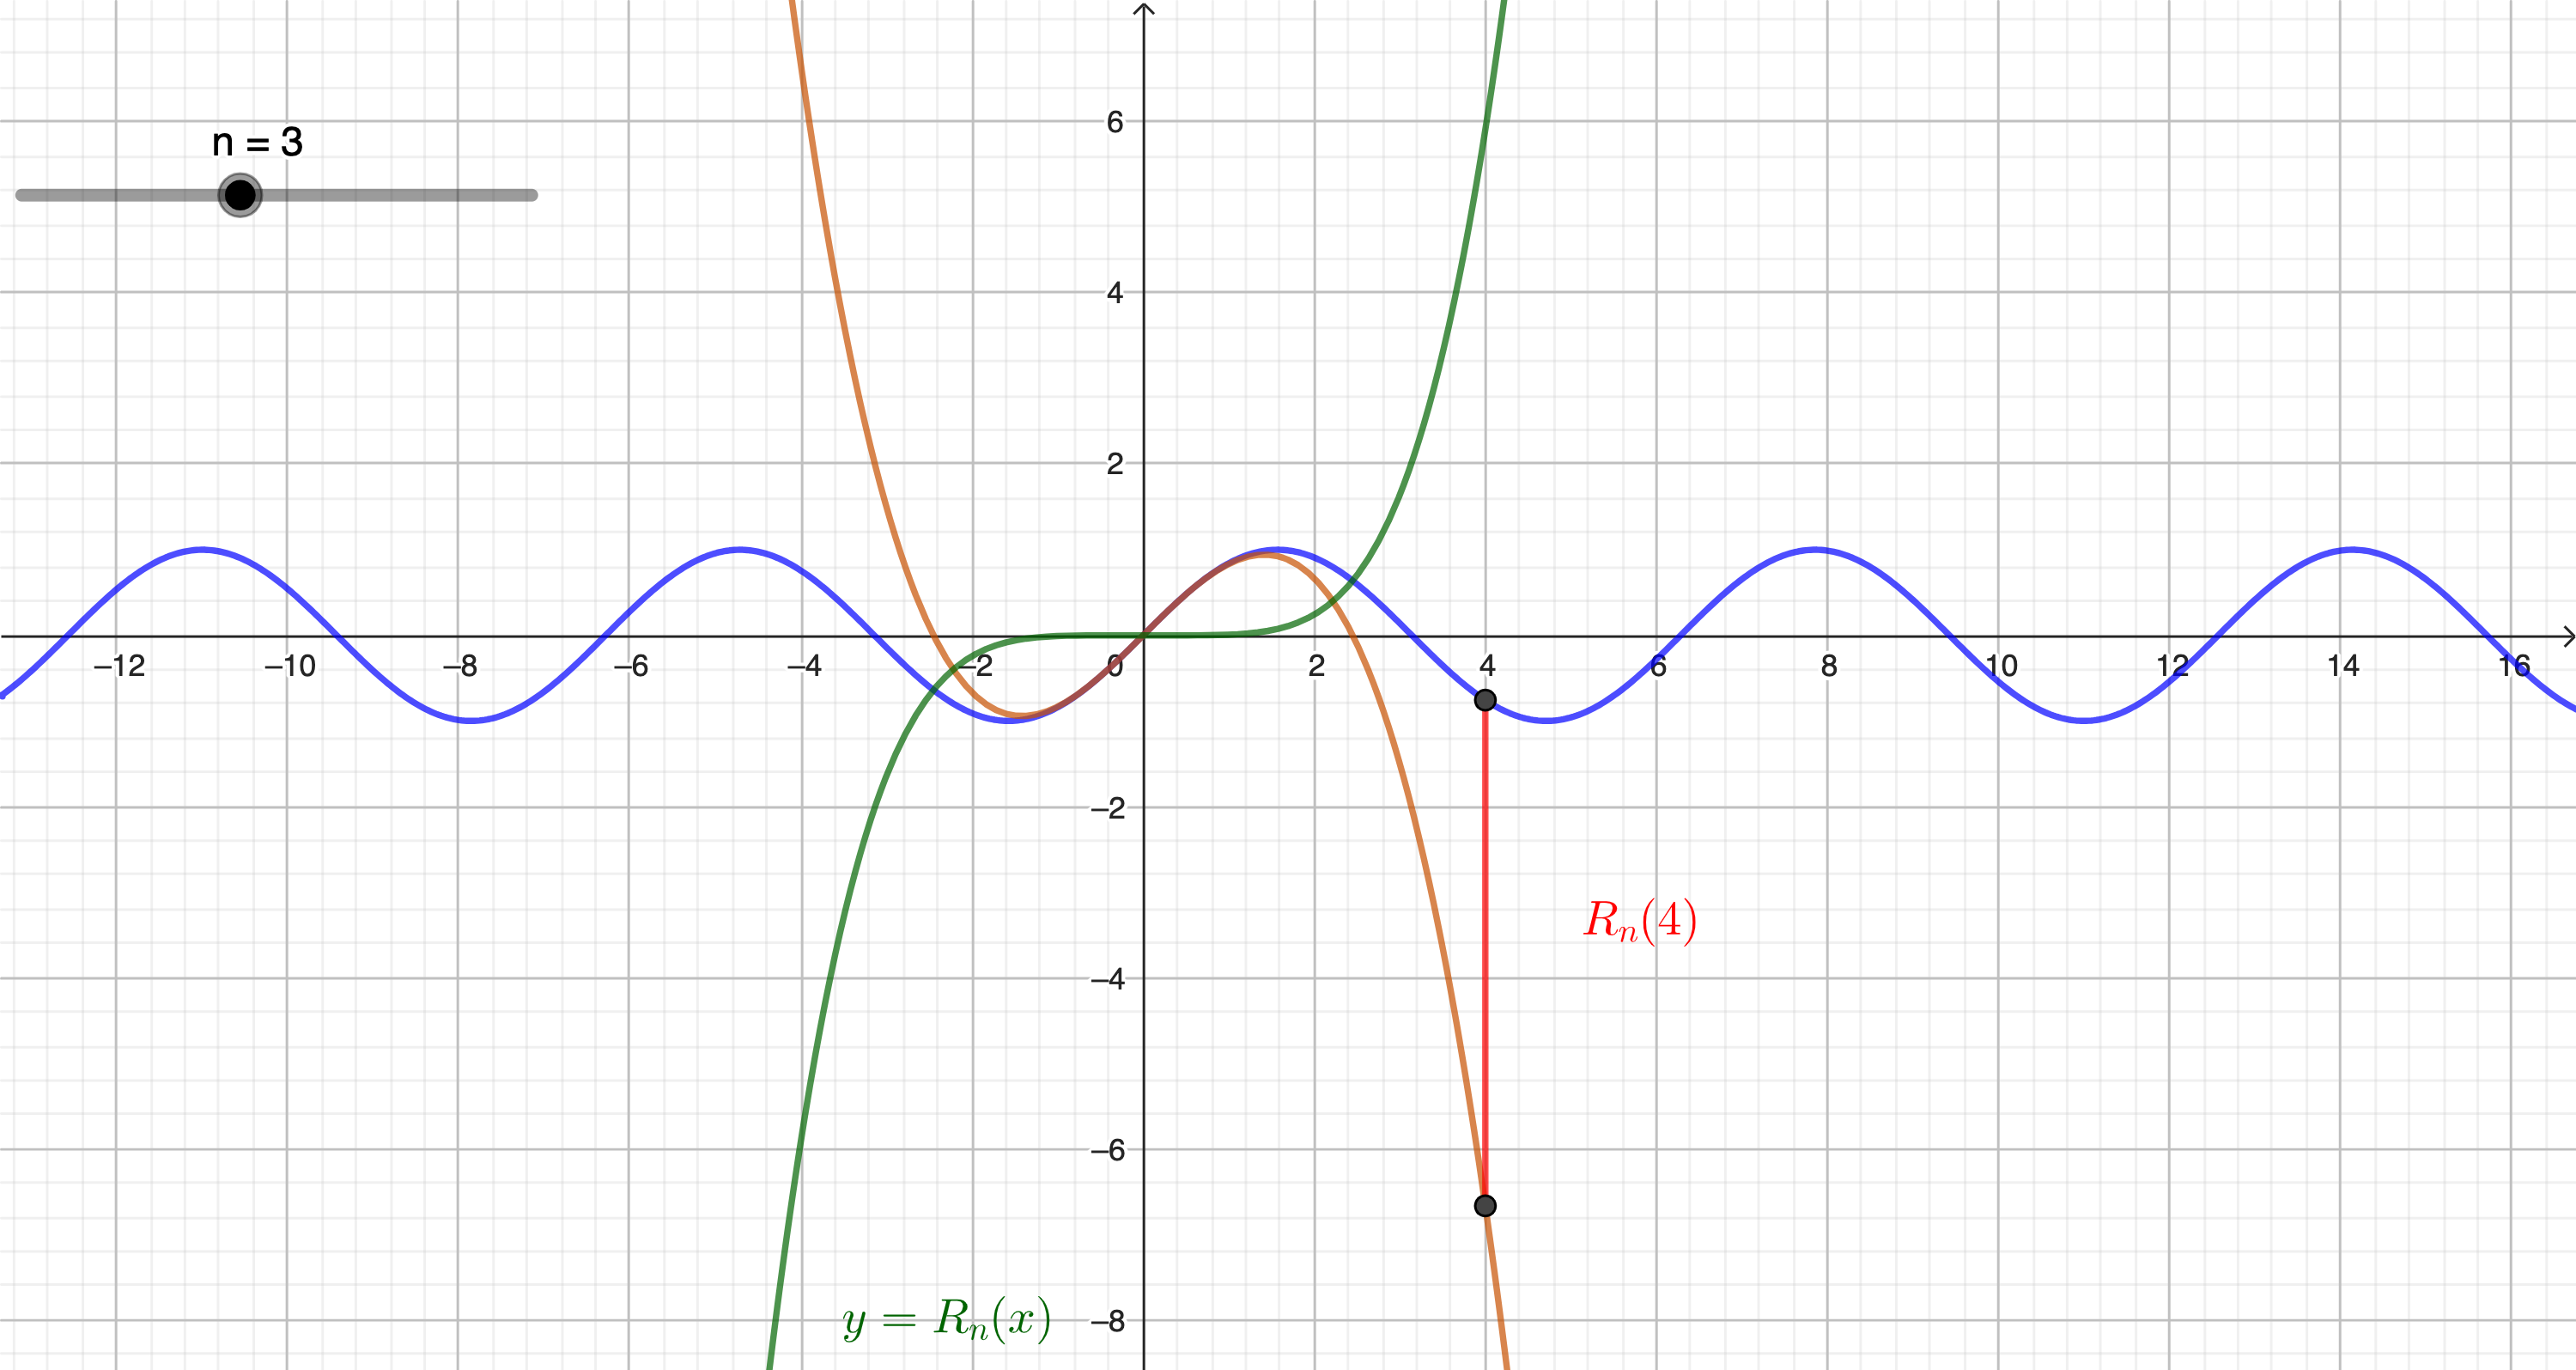
\includegraphics[width=0.45\textwidth]{media/restglied3.png}

	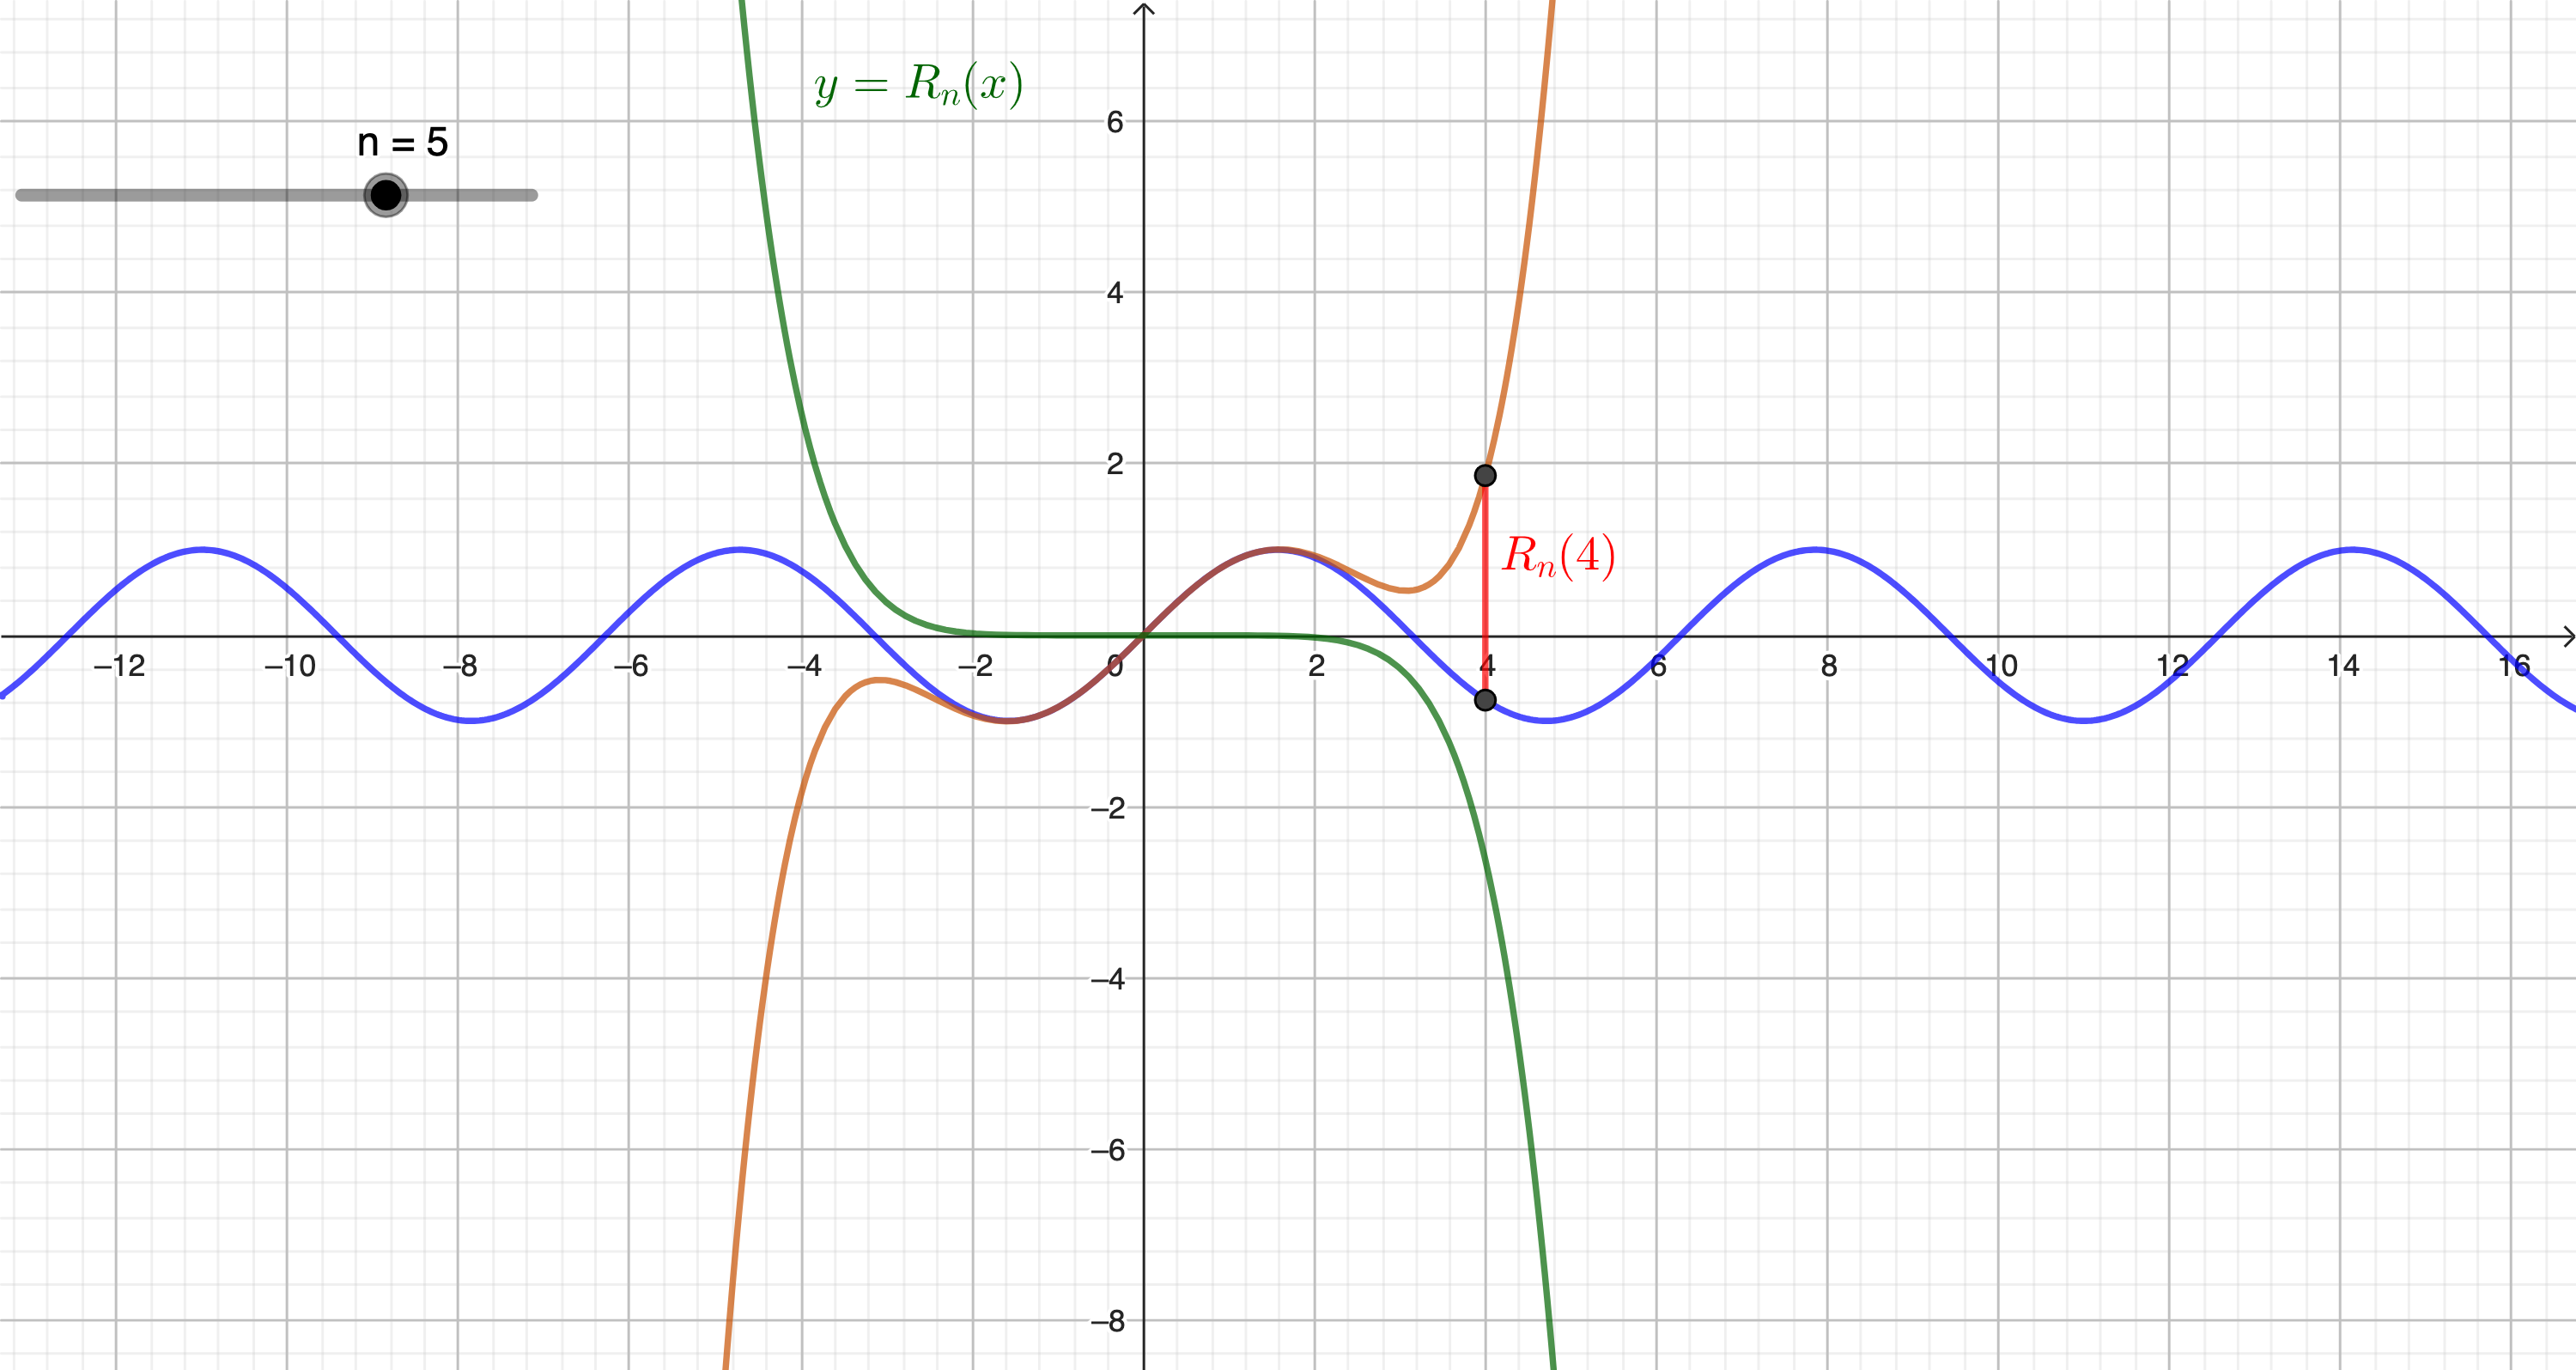
\includegraphics[width=0.45\textwidth]{media/restglied5.png}
	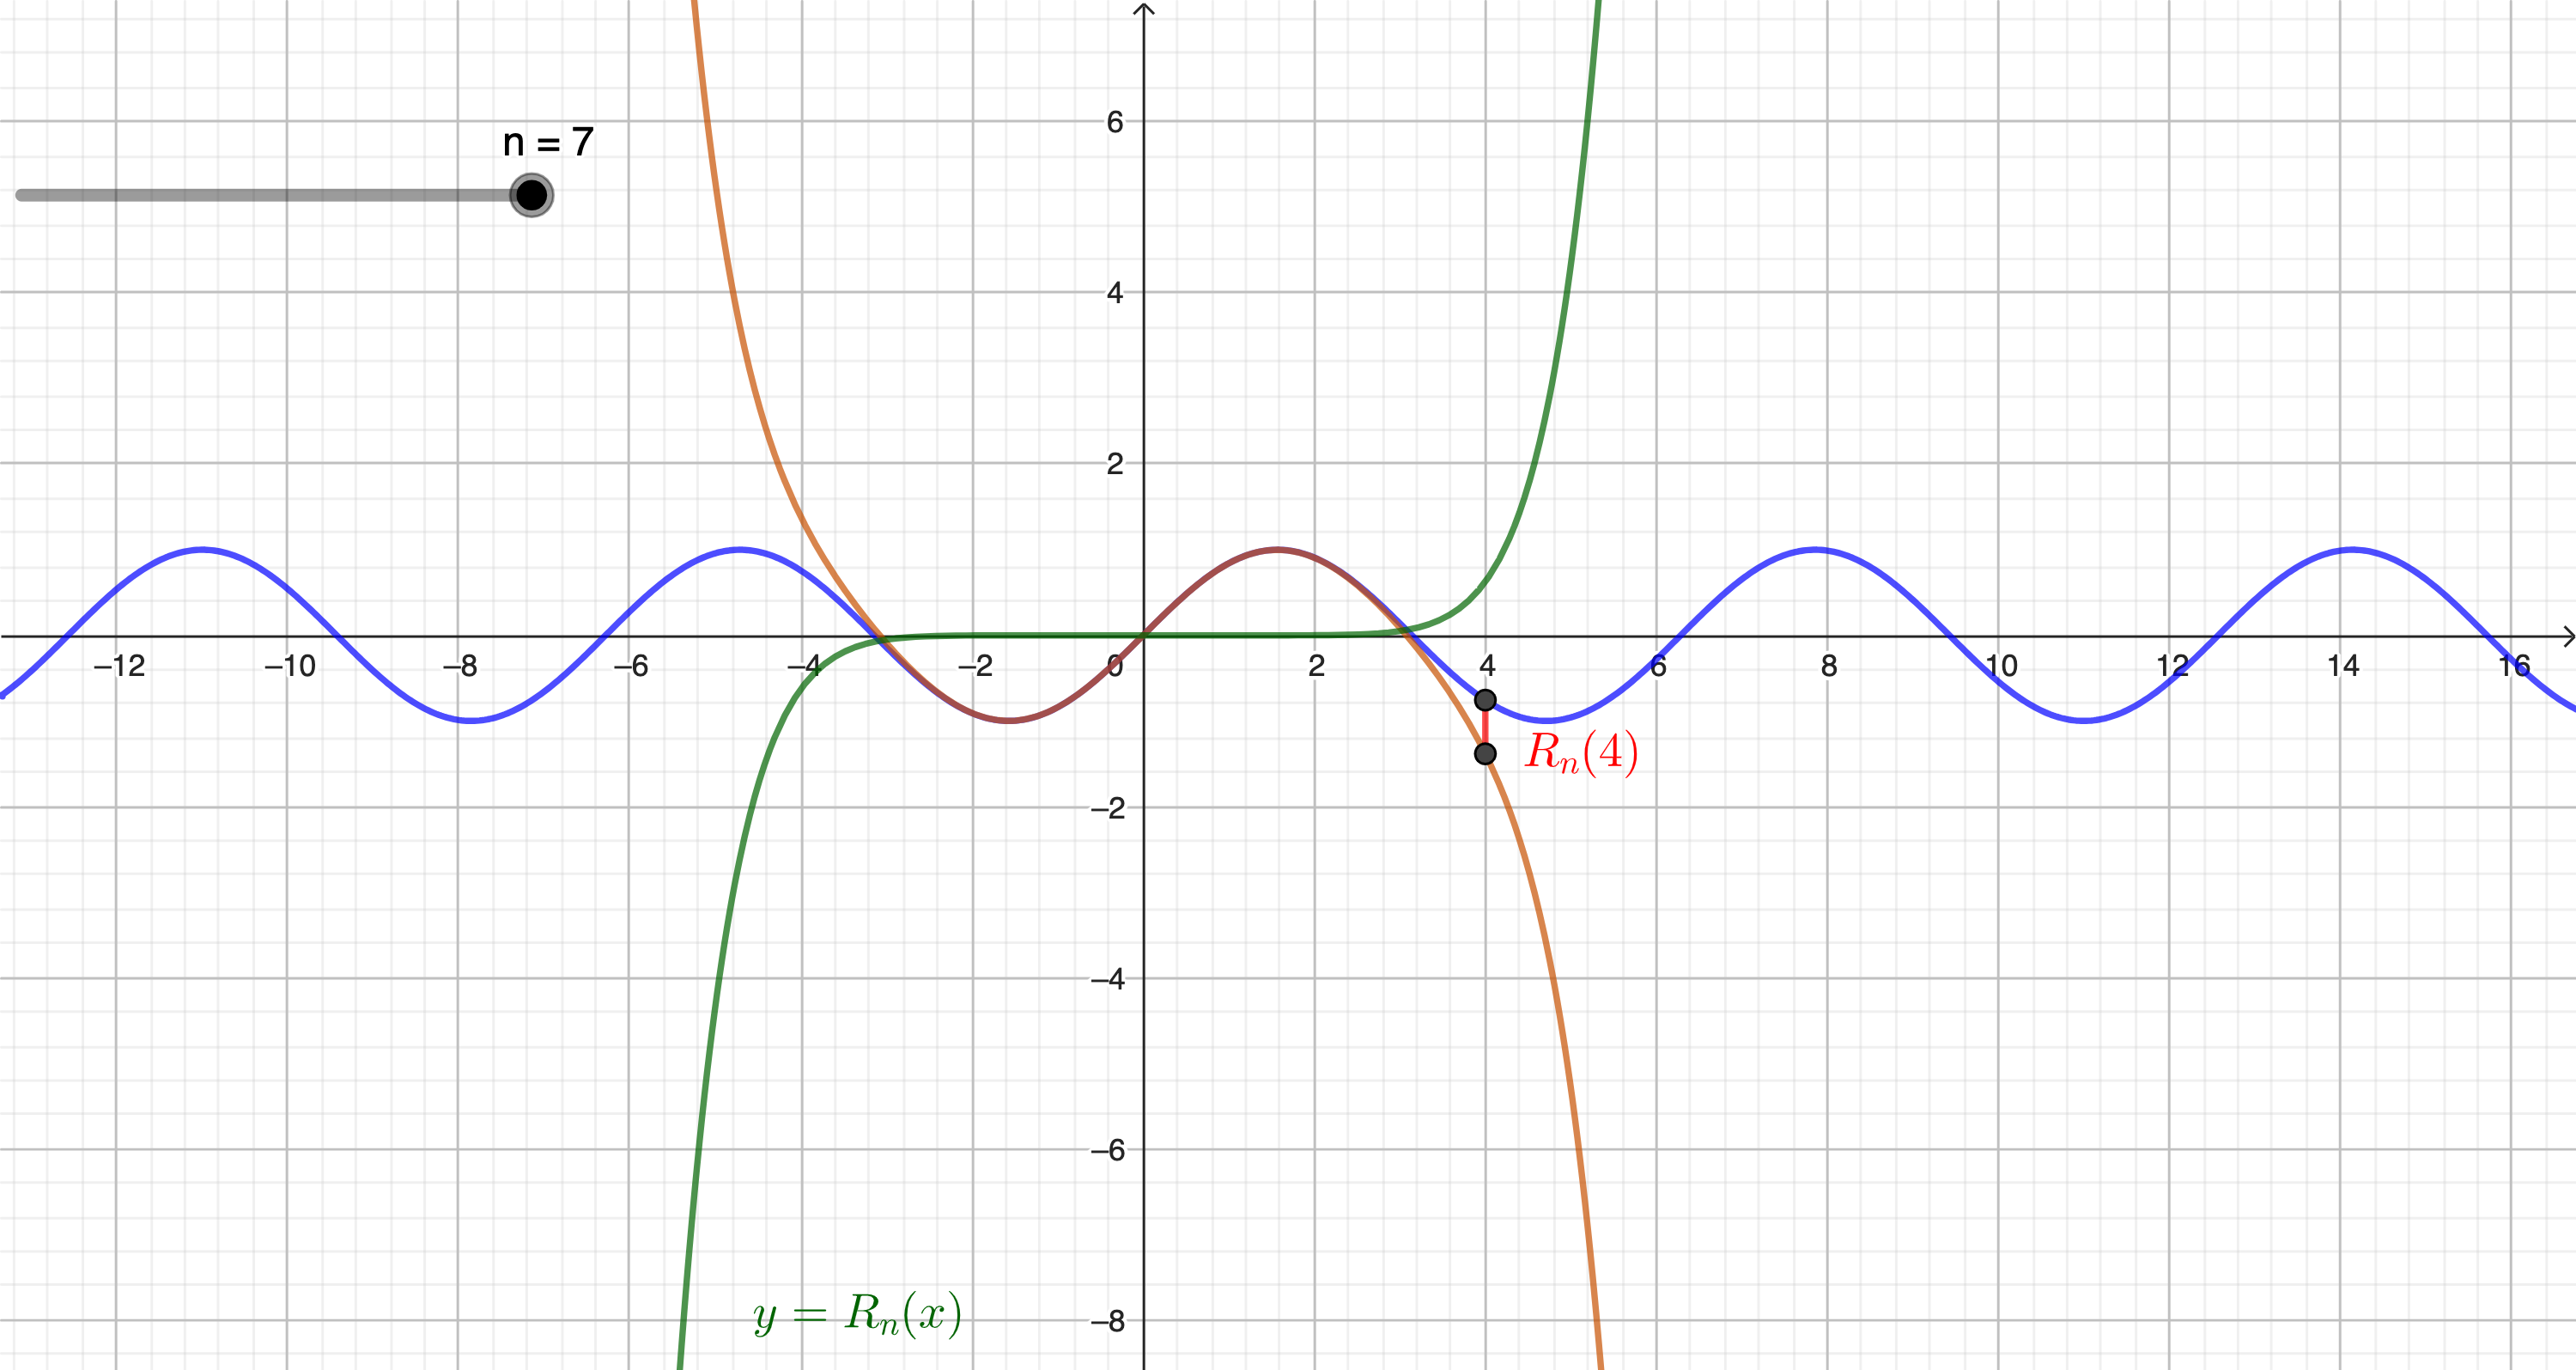
\includegraphics[width=0.45\textwidth]{media/restglied7.png}
	\caption{Restglied der Sinusfunktion für $n=1, 3, 5, 7$}
\end{figure}


Im Idealfall strebt die Abweichung $R_n(x)$ zwischen der Funktion $f$ und deren Taylorpolynom $T_n(x)$ für jeden Wert von $x$ gegen $0$.  Das ist bei der Sinusfunktion tatsächlich der Fall.

Um dies nachvollziehen zu können, werden wir den folgenden Weg beschreiten:
\begin{enumerate}
	\item Wir lernen den ersten Mittelwertsatz der Differentialrechnung kennen. Dabei handelt es sich um einen sogenannten Existenzsatz. Wir werden aber sehen, wie man aus solchen Sätzen konkrete Schlüsse ziehen kann.
	\item Mit dem  Mittelwertsatz werden wir eine Formel für die Berechnung des Restglieds $R_n(x)$ herleiten können. Damit lässt sich berechnen, wie genau eine Approximation durch ein Taylorpolynom ist.
	\item Schliesslich werden wir untersuchen, wie sich die Formel für das Restglied $R_n(x)$ verhält, wenn $n$ immer grösser wird. Damit können wir Beweisen, dass die Taylorreihen von $e^x, \sin(x), \cos(x)$ für $n\to\infty$ an jeder Stelle gegen die entsprechende Funktion konvergiert.
\end{enumerate}


